\documentclass[a4paper, 12pt]{article}

% --- Pacchetti Fondamentali ---
\usepackage{amsmath}
\usepackage{float}    % Per forzare il posizionamento con [H]
\usepackage[utf8]{inputenc}     % Codifica caratteri
\usepackage[T1]{fontenc}        % Codifica font
\usepackage[italian]{babel}     % Lingua italiana
\usepackage{geometry}           % Gestione margini
\geometry{a4paper, margin=2.5cm}
\usepackage{lmodern}            % Font leggibile
\usepackage{enumitem}           % Per liste personalizzate
\usepackage{graphicx}
\usepackage{listings}
\usepackage{microtype}
\usepackage{helvet} %responsabile 1 per il cambio di stile di puntegiatura 
% --- Pacchetti per Tabelle e Grafica ---
\usepackage{tabularx}
\usepackage{longtable}          % Per tabelle multipagina
\usepackage{booktabs}           % Per linee tabella professionali
\usepackage{array}              % Per gestione colonne
\usepackage[dvipsnames]{xcolor}             % Per colori
\usepackage{titlesec}           % Per formattazione titoli
\usepackage{hyperref}           % Per link e indice
\newcommand{\req}[1]{\hyperref[req:#1]{#1}}
% --- Configurazione Link e Colori ---
\definecolor{linkblue}{RGB}{0, 102, 204}
\definecolor{headergray}{RGB}{240, 240, 240}

\hypersetup{
    colorlinks=true,
    linkcolor=black,        % Nero nell'indice per eleganza
    urlcolor=linkblue,
    pdftitle={Mobile MealMate},
}



\definecolor{promptcolor}{HTML}{A6E22E} % Monokai Green
\definecolor{Greenm}{rgb}{109,245,94}

\renewcommand{\familydefault}{\sfdefault} %responsabile 2 per il cambio di stile di puntegiatura 

\begin{document}

% --- FRONTESPIZIO ---
% Title Page
\begin{titlepage}
    \begin{center}
        % University Logo
        
\includegraphics[width=0.3\textwidth]{immage/logo_standard.png}\\[1cm]
        
        {\Huge\textbf{Università degli Studi di Salerno}}\\[0.5cm]
        {\Large\textbf{Dipartimento di Ingegneria dell’Informazione ed Elettrica e Matematica applicata}}\\[1.5cm]

        % Relazione tecnica
        {\Large\textbf{Relazione Tecnica di Progettazione e Sviluppo}}\\[0.5cm]
        {\large\textbf{Progetto di Mobile Programming}}\\[1.5cm]
        
        % Nome programma
        {\Large \textbf{{MealMate}}}\\[0.2 cm]
        {\large \textbf{\textit{Meal Planner e Smart Pantry App}}}\\[3cm]
        
        % Thesis Title
        %PROGETTAZIONE E SVILUPPO DI UNA PIATTAFORMA DIGITALE PER LA GESTIONE DELLE PRENOTAZIONI. 
        {\large \textit{Tecnologie utilizzate: Dart • Flutter • SQLite -SharedPreferences}}\\[0.5cm]
        {\large \textbf{}}\\[1cm]
        \end{center}
        
        \noindent
    
    \hfill
    \begin{minipage}[t]{0.48\textwidth}
        \raggedleft
        \textbf{Gruppo 17:} \\
        \textit{{Ercolano Aniello}}\\
        \textit{{Cangianiello Francesco}}\\
        \textit{{Giannitti Serena}}\\
        \textit{{Rossomando Andrea}}\\
    \end{minipage}
    
    \vfill
    % Academic Year
    \begin{center}
        {\large Anno Accademico 2025/2026}\\[0.5cm]
        \end{center}
\end{titlepage}

\newpage
\tableofcontents
\newpage
%----sezione 1----
\section{Descrizione dell’applicazione}
\subsection{Obiettivo}
“MealMate” è un’applicazione mobile sviluppata in Flutter che ha lo scopo di supportare l’utente nella gestione quotidiana della propria alimentazione.\\
L’app integra in un’unica piattaforma la pianificazione dei pasti e la gestione delle ricette, di una dispensa virtuale dove catalogare ingredienti e prodotti disponibili e di una lista della spesa.\\
L’app nasce dalla necessità di centralizzare queste attività, le quali normalmente vengono gestite in modo frammentato. \textbf{MealMate} unifica tutto in un’unica esperienza coerente.

\subsection{Target Audience}
La strategia adottata per definire il target di riferimento è la segmentazione comportamentale. Si definiscono tre principali personas, 
ovvero tre modelli di utenti in base al motivo per cui utilizzeranno l’applicazione:
\begin{itemize}
    \item Studenti e Giovani Professionisti. Utenti che vivono da soli o con dei coinquilini, con ritmi elevati e risorse economiche da gestire
    \item Atleti Amatoriali e Professionisti. Utenti che tengono al loro stile di vita e che seguono una dieta precisa
    \item Famiglie e Genitori Lavoratori. Utenti che devono gestire l’alimentazione di un gruppo familiare, con poco tempo a disposizione.
\end{itemize}
Questi gruppi rappresentano i principali target di riferimento dell’applicazione, ma non sono esaustivi.

\subsection{Problemi risolti dall’applicazione}
L’applicazione intende risolvere diversi problemi
\begin{itemize}
    \item \textbf{Dispersione delle informazioni}: ricette, ingredienti e liste sparse su più supporti.
    \item \textbf{Mancanza di pianificazione}: l’app presenta un’organizzazione anticipata dei pasti grazie alla programmazione settimanale.
    \item \textbf{Inefficienza nella spesa}: acquisto di prodotti già disponibili o mancanza di ingredienti necessari.
    \item \textbf{Gestione migliore della distribuzione economica}, grazie alle liste della spesa.
    \item \textbf{Sprechi alimentari}.
\end{itemize}

% ----- sezione casi d'uso ---- 
\newcounter{cp}
\setcounter{cp}{1}  
\renewcommand{\count}{ \arabic{cp} \stepcounter{cp} }  

\newpage
\subsection{Principali scenari d’uso}
{\large\textbf{UC-\count} \hspace{0.5 cm}   \textbf{Aggiunta ricetta}}
\begin{enumerate}[label=\arabic*.]
    \item L’utente entra nel menù \textbf{Ricette} e clicca sul tasto +.
    \item L’utente inserisce il nome della ricetta, il procedimento, la categoria, il tempo di preparazione, la difficoltà, le porzioni, gli ingredienti ed eventuali note e una foto.
    \item L’utente clicca sul tasto \textbf{"salva"} per salvare la ricetta e poterla ricercare. 
\end{enumerate}

\vspace{0.5 cm}
\hrule
\vspace{0.5 cm}

\raggedright{\large\textbf{UC-\count} \hspace{0.5 cm} \textbf{Aggiunta ricetta ai preferiti}}\\[0.5 cm]
\textbf{Precondizioni:} l’utente ha inserito almeno una ricetta
\begin{enumerate}[label=\arabic*.]
    \item L’utente entra nel menù \textbf{Ricette}
    \item L’utente clicca sul pulsante a forma di cuore presente sulla ricetta per aggiungerla ai preferiti e visualizzarla in una schermata separata.
\end{enumerate}

\vspace{0.5 cm}
\hrule
\vspace{0.5 cm}

{\large\textbf{UC-\count} \hspace{0.5 cm}   \textbf{Dispensa}}
\begin{enumerate}[label=\arabic*.]
    \item L’utente entra nel menù \textbf{Dispensa} e visualizza la lista di prodotti già in dispensa, ricerca un prodotto o aggiunge un nuovo prodotto cliccando sul tasto verde +.
    \item Cliccando il "tasto verde", l’utente può inserire il nome del prodotto, la categoria, la quantità, l’unità di misura, eventuali note e la data di scadenza, scegliendo da un calendario.
    \item L’utente clicca sul tasto salva per salvare il prodotto nella dispensa
\end{enumerate}

\vspace{0.5 cm}
\hrule
\vspace{0.5 cm}

{\large\textbf{UC-\count} \hspace{0.5 cm}   \textbf{Meal Plan}}
\begin{enumerate}[label=\arabic*.]
    \item L’utente entra nel menù \textbf{Meal Plan} e visualizza un elenco di pasti pianificati.
    \item L’utente può scegliere la settimana, il tipo del pasto e la ricetta per preparare un meal plan.
    \item L’utente può cliccare sul tasto “aggiungi al piano” per aggiungere il meal plan all’elenco di pasti pianificati
\end{enumerate}

\newpage

{\large\textbf{UC-\count} \hspace{0.5 cm}   \textbf{Lista Spesa}}
\begin{enumerate}[label=\arabic*.]
    \item L’utente entra nel menù \textbf{Lista Spesa} e visualizza la lista della spesa, se presente.
    \item L’utente scrive il nome di un prodotto, la quantità e l’unità di misura nei rispettivi campi e, cliccando sul tasto verde +, inserisce il prodotto nella lista.
    \item[] \textbf{Flusso alternativo}
    \begin{enumerate}
    \item[2a.] L’utente clicca sul tasto Genera dal Meal Plan per generare automaticamente la lista della spesa sulla base dei pasti preparati.
    \end{enumerate}
\end{enumerate}

\vspace{0.5 cm}
\hrule
\vspace{0.5 cm}

{\large\textbf{UC-\count} \hspace{0.5 cm}   \textbf{Statistiche}}
\begin{enumerate}[label=\arabic*.]
    \item L’utente entra nel menù \textbf{Statistiche}
    \item Vengono visualizzate diverse informazioni, tra cui le ricette salvate, i prodotti in dispensa, i pasti pianificati, il numero di prodotti nella lista della spesa, il tempo medio di preparazione, i prodotti vicini alla scadenza, i prodotti scaduti. Permette inoltre di visualizzare le ricette preferite.
\end{enumerate}


%---- Requisiti ----
\newpage
\section{Requisiti}
\subsection{Funzionalità implementate}

{\color{ForestGreen}\raggedright{\large \textbf{Gestione Ricette}}}
\begin{itemize}
    \item Visualizzazione elenco ricette con ricerca per nome o categoria e filtro per categoria.
    \item Schermata di dettaglio con immagine, ingredienti, procedimento, tempi e difficoltà.
    \item Eliminazione ricetta (con rimozione automatica dal meal plan associato).
    \item Inserimento, modifica ed eliminazione di ricette tramite form completo con aggiunta dinamica di ingredienti.
    \item Marcatura come preferita e schermata dedicata alle ricette preferite con filtri avanzati.
    \item Sezione “Consigliate da noi” che suggerisce alcune ricette hardcoded dagli sviluppatori e altre in base agli ingredienti e alle relative quantità disponibili in dispensa.
\end{itemize}

\vspace{0.5 cm}
\hrule
\vspace{0.5 cm}

{\color{ForestGreen}\raggedright{\large \textbf{Gestione Dispensa}}}
\begin{itemize}
    \item Visualizzazione con ricerca per nome e categoria.
    \item Raggruppamento automatico in: Prodotti Scaduti, In Scadenza (entro 3 giorni), Altri Prodotti.
    \item Form completo per aggiunta e modifica con selezione data di scadenza tramite date picker.
    \item Selezione unità di misura da lista predefinita con opzione personalizzata.
    \item Eliminazione con bottone dedicato.
\end{itemize}

\vspace{0.5 cm}
\hrule
\vspace{0.5 cm}

{\color{ForestGreen}\raggedright{\large \textbf{Pianificazione Pasti (Meal Plan)}}}
\begin{itemize}
    \item Vista settimanale con espansione per giorno.
    \item Aggiunta pasto con selezione giorno, tipologia (Colazione/Pranzo/Cena/Spuntino) e ricetta
    \item Rimozione di singoli pasti pianificati.
    \item Contatore pasti per ogni giorno.
\end{itemize}

\newpage

{\color{ForestGreen}\raggedright{\large \textbf{Lista della Spesa}}}
\begin{itemize}
    \item Aggiunta manuale di prodotti con nome, quantità e unità di misura.
    \item Generazione automatica dal meal plan (escludendo prodotti già in dispensa).
    \item Aggregazione intelligente:
    \begin{itemize}[label=•]
        \item prodotti identici con stessa unità vengono sommati.
        \item prodotti identici con unità diverse non vengono sommati (l’utente potrebbe volere un determinato prodotto in formati differenti).
    \end{itemize}

    \item Spunta come acquistato, selezione multipla ed eliminazione in blocco.
    \item Dialog per aggiungere il prodotto acquistato direttamente in dispensa.
\end{itemize}

\vspace{0.5 cm}
\hrule
\vspace{0.5 cm}

{\color{ForestGreen}\raggedright{\large \textbf{Statistiche}}}
\begin{itemize}
    \item Contatori: ricette, prodotti dispensa, pasti pianificati, elementi lista spesa, prodotti in scadenza, prodotti scaduti, tempo medio di preparazione delle ricette.
    \item Elenco prodotti in scadenza e scaduti con indicatori visivi.
    \item Accesso rapido alle ricette preferite con contatore.
\end{itemize}

\newpage

\subsection{Funzionalità considerate e non implementate}
\begin{itemize}
    \item Gestione nutrizionale (calorie, macronutrienti) per limitare il perimetro del progetto.
    \item Importazione ricette da URL o servizi esterni.
    \item Integrazione dell'API di Google Calendar per consigliare piatti tipici durante le festività.
\end{itemize}


\subsection{Feature avanzate scelte}
\begin{itemize}
    \item Ricette consigliate: il menù Ricette visualizza in una sezione le ricette consigliate in base alla disponibilità degli ingredienti nella dispensa.
    \item Generazione automatica Lista Spesa: nel menù Lista Spesa è possibile far generare all’applicazione una lista sulla base del Meal Plan preparato.
    \item Gestione avanzata delle scadenze con tre livelli di allerta visiva (scaduto, in scadenza, a norma) e ordinamento per data. Sia la sezione Statistiche dell’applicazione sia la sezione Dispensa tengono traccia dei prodotti vicini alla scadenza e dei prodotti scaduti. 
\end{itemize}

\subsection{Eventuali limitazioni note}
\begin{itemize}
    \item La gestione delle unità di misura non include conversioni automatiche (es. g → kg): la corrispondenza avviene per stringa esatta.
    \item Le immagini delle ricette vengono salvate con il percorso assoluto locale, quindi non sono portabili tra dispositivi diversi.
\end{itemize}

\newpage

% --- section 3 Progettazione ---

\section{Progettazione}
\subsection{Struttura generale}
L’app è strutturata in tre livelli architetturali distinti:
\begin{itemize}
    \item \textbf{Presentazione} (UI Layer): schermate Flutter e widget riutilizzabili.
    \item \textbf{Stato e logica} (State Layer): AppState gestisce lo stato globale e le operazioni sui dati.
    \item \textbf{Persistenza} (Data Layer): DatabaseHelper per SQLite (ricette) e SharedPreferences per gli altri dati.
\end{itemize}

\vspace{0.5 cm}
L’applicazione si suddivide in 5 sezioni principali:
\begin{itemize}
    \item La sezione \textbf{Ricette} permette di cercare, aggiungere o rimuovere una ricetta, aggiungere o rimuovere una ricetta dai preferiti, visualizzare la lista di ricette, la lista di ricette preferite e la lista di ricette consigliate dalla dispensa.
    \item La sezione \textbf{Dispensa} permette di cercare, aggiungere o rimuovere un prodotto e di visualizzare la lista dei prodotti.
    \item La sezione \textbf{Meal Plan} permette di pianificare i pasti di ogni giorno scegliendo una ricetta e di visualizzare i pasti pianificati.
    \item La sezione \textbf{Lista Spesa} permette di aggiungere o rimuovere uno o più elementi dalla lista e di visualizzare la lista della spesa. Permette inoltre di generare una lista automaticamente dal meal plan.
    \item La sezione \textbf{Statistiche} visualizza una serie di statistiche relative alle ricette salvate, ai pasti pianificati, ai prodotti in scadenza o scaduti, alle ricette preferite e calcola il tempo medio di preparazione delle ricette salvate.    
\end{itemize}

% --- tabella ----
\subsection{Schermate principali}
\begin{table}[H]
    \centering
    \renewcommand{\arraystretch}{1.5}
    \begin{tabularx}{\textwidth}{@{} >{\bfseries}l X @{}}
        \toprule
        \textbf{Schermata} & \textbf{Descrizione} \\
        
        \midrule
        HomeScreen & Schermata di benvenuto con griglia di accesso rapido alle sezioni \\
        \addlinespace
        RecipesScreen & Elenco ricette con ricerca, filtri per categoria e sezione “Consigliate” a scorrimento orizzontale \\
        \addlinespace
        RecipeDetailScreen & Dettaglio ricetta con header immagine, informazioni aggiuntive, ingredienti e procedimento \\
        \addlinespace
        RecipeFormScreen & Form di inserimento/modifica con righe ingredienti e selezione immagine dalla galleria \\
        \addlinespace
        FavoriteRecipesScreen & Lista preferiti con filtri avanzati per categoria, difficoltà e tempo di preparazione \\
        \addlinespace
        PantryScreen & Dispensa con raggruppamento automatico per stato scadenza e ricerca full-text \\
        \addlinespace
        PantryFormScreen & Form aggiunta/modifica prodotto con date picker e dropdown unità di misura \\
        \addlinespace
        MealPlanScreen & Pianificazione settimanale con vista a fisarmonica per giorno \\
        \addlinespace
        ShoppingListScreen & Lista della spesa con aggiunta manuale, generazione automatica e dialog di trasferimento in dispensa \\
        \addlinespace
        StatsScreen & Statistiche e riepilogo con indicatori visivi per prodotti in scadenza e scaduti \\
        
        \bottomrule
    \end{tabularx}
    \caption{Schermate principali dell'applicazione}
    \label{tab:requisiti_sistema}

\end{table}
\newpage


\subsection{Wireframe}
In questa sezione vengono presentati i \textbf{wireframe} preliminari progettati per lo sviluppo dell'applicazione mobile. \\
Questi schemi, affinati attraverso diverse iterazioni, hanno fornito una fondamentale linea guida visiva e strutturale, fungendo da base per l'implementazione dell'interfaccia utente (UI) e della logica applicativa di ogni schermata.

\begin{figure}[H]
    \vspace{2 cm}
    \centering
    \begin{minipage}{0.45\textwidth}
        \centering
        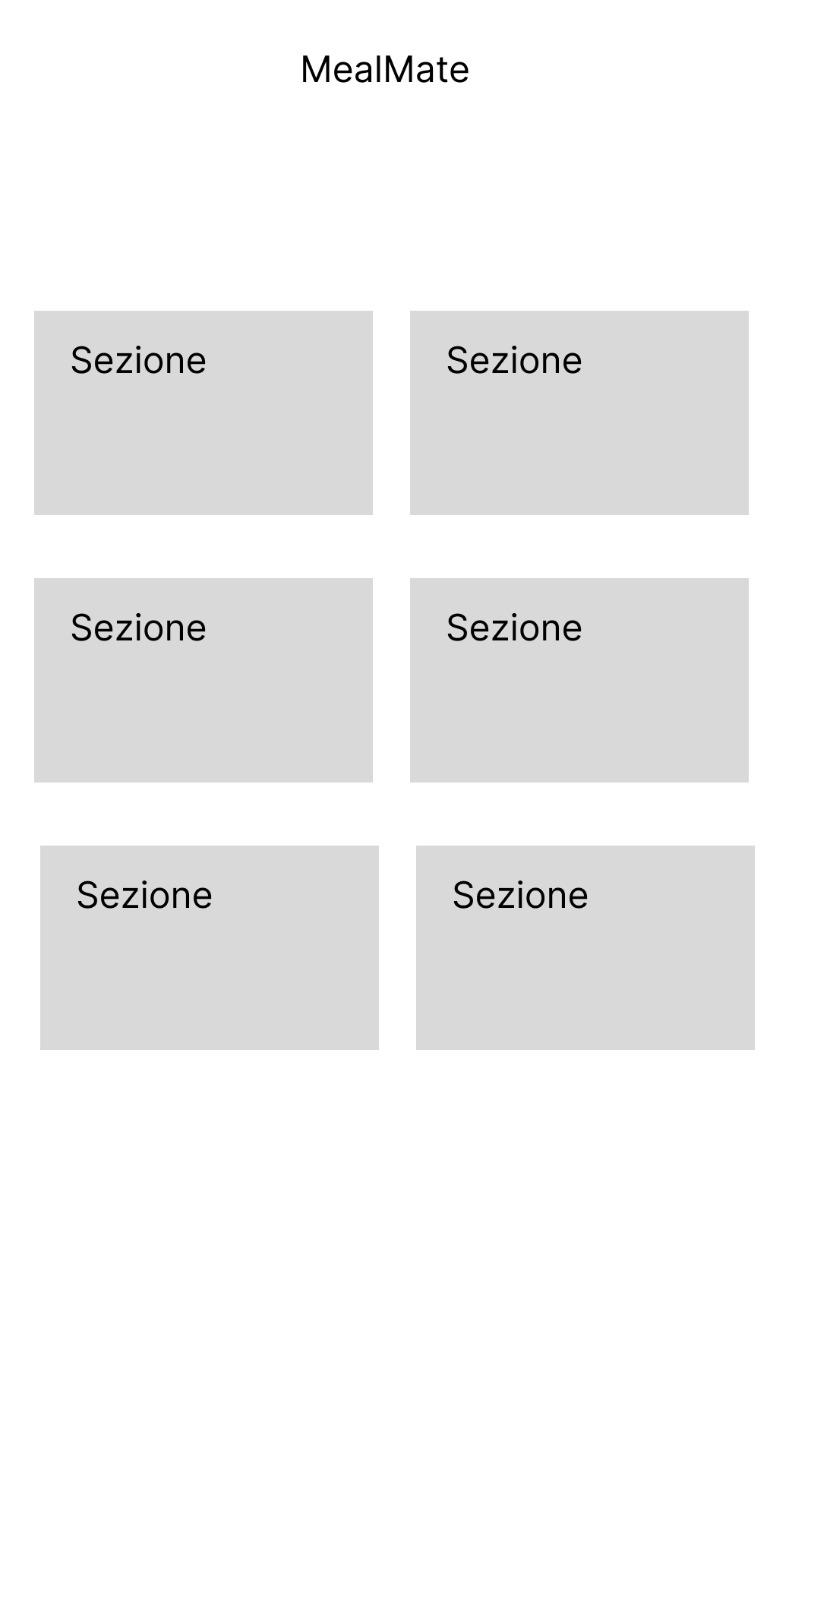
\includegraphics[width=\textwidth]{immage/home.jpeg}
        \caption{Wireframe della home page}
    \end{minipage}
    \hfill
    \begin{minipage}{0.45\textwidth}
        \centering
        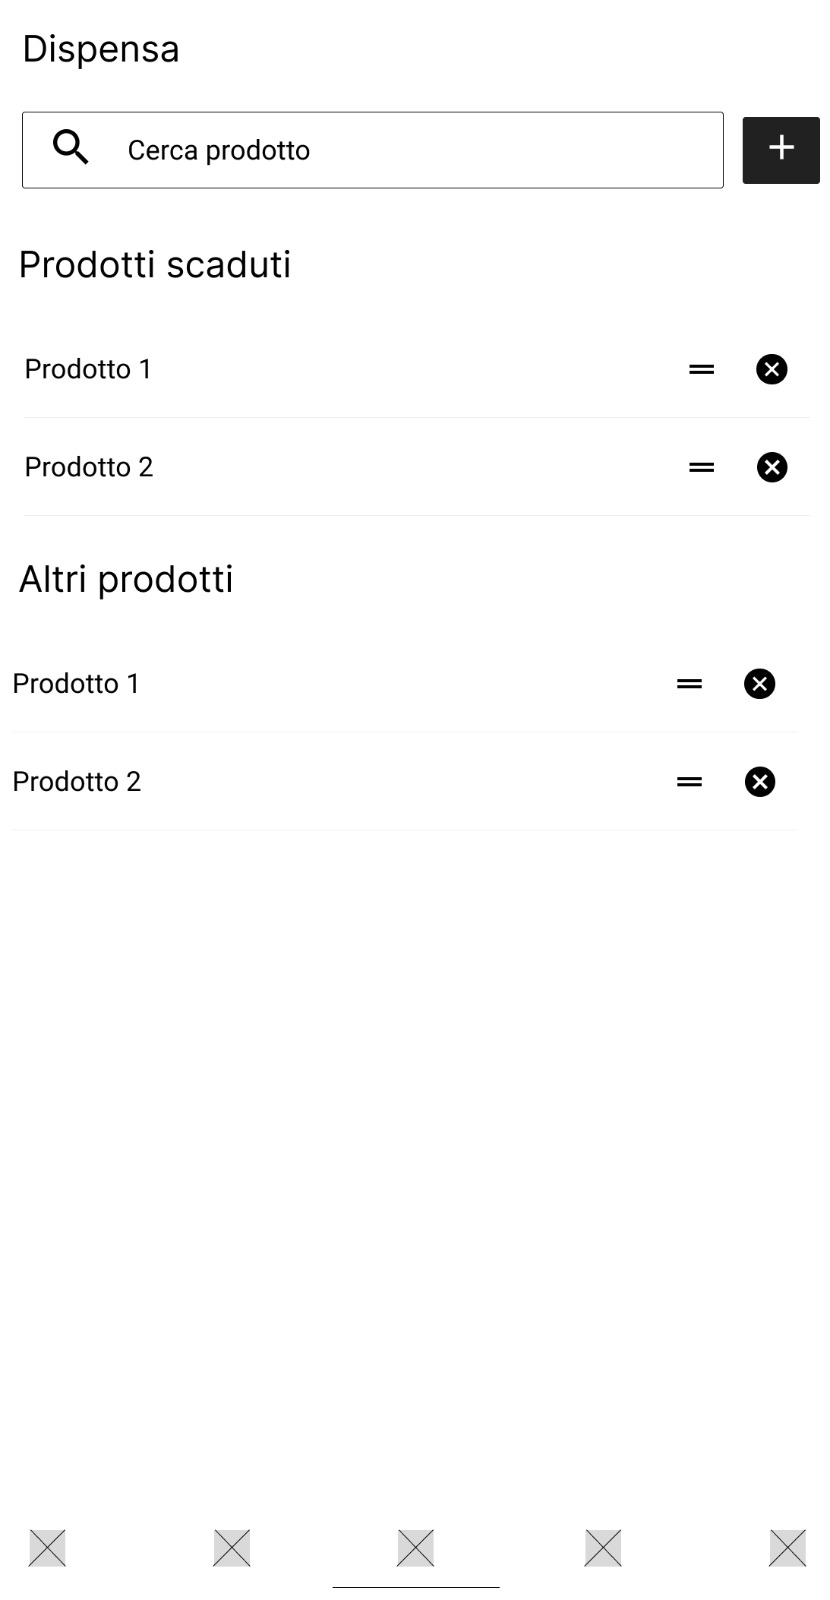
\includegraphics[width=\textwidth]{immage/Dispensa.jpeg}
        \caption{Wireframe di Dispensa}
    \end{minipage}
\end{figure}

\newpage
\begin{figure}[H]
    \centering
    \vspace{3 cm}
    \begin{minipage}{0.45\textwidth}
        \centering
        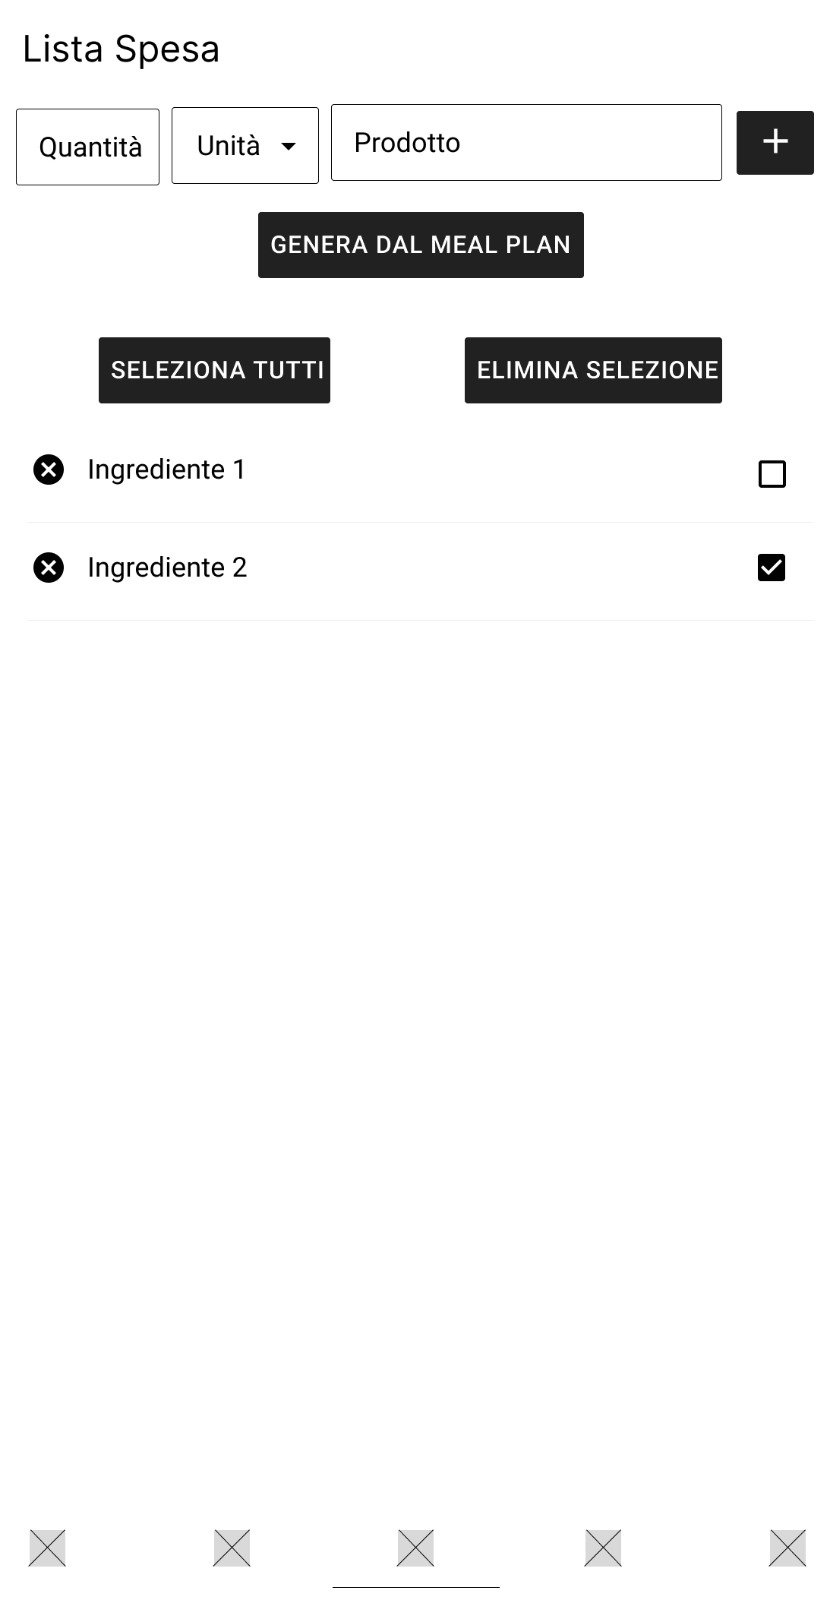
\includegraphics[width=\textwidth]{immage/Lista-spesa.jpeg}
        \caption{Wireframe di Lista-spesa}
    \end{minipage}
    \hfill
    \begin{minipage}{0.45\textwidth}
        \centering
        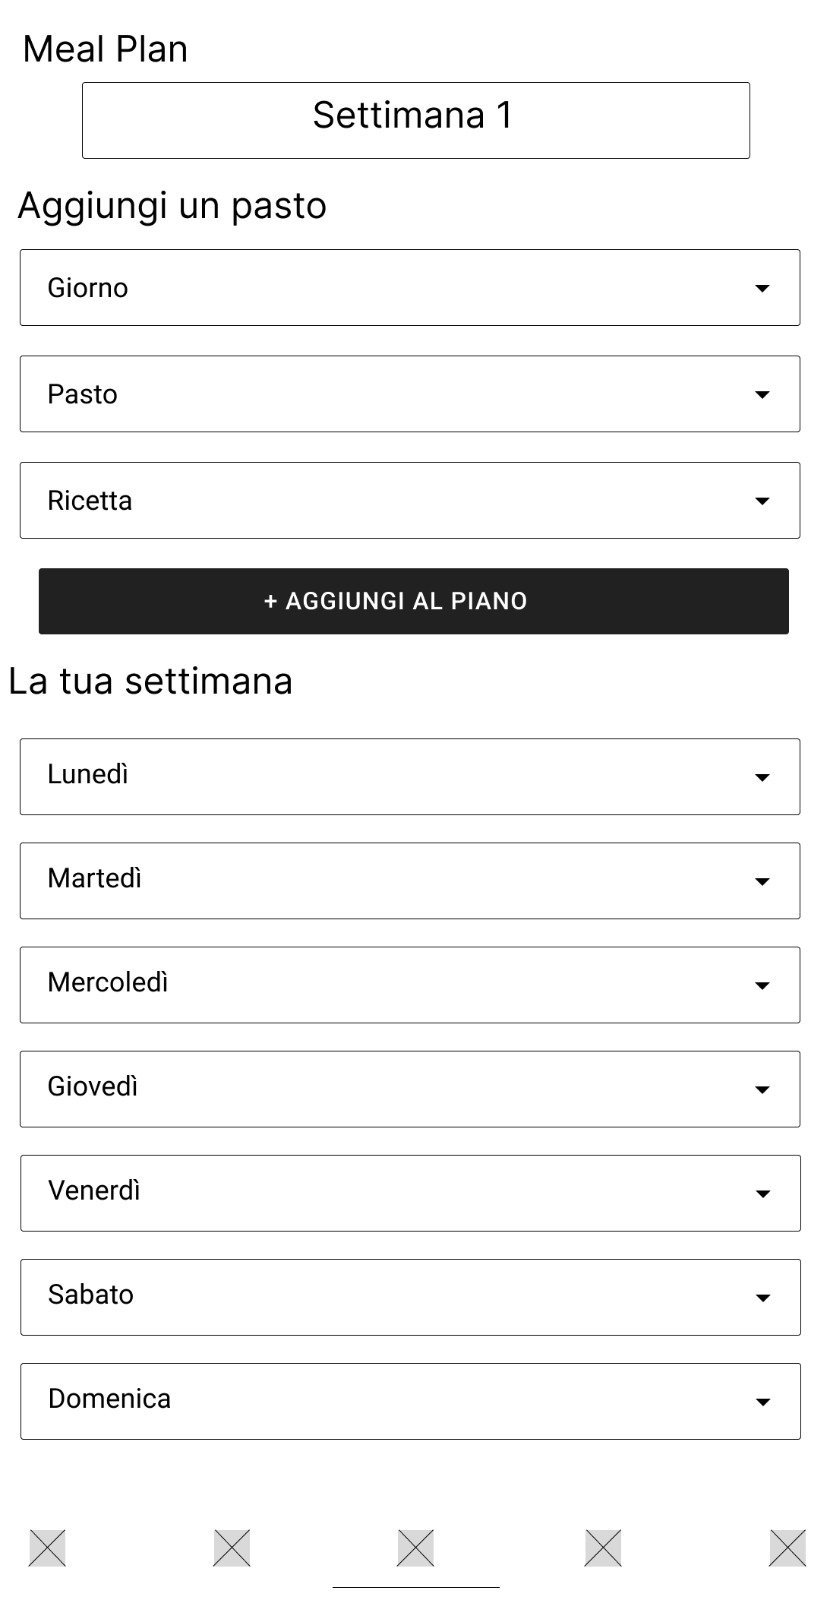
\includegraphics[width=\textwidth]{immage/Meal-Plean.jpeg}
        \caption{Wireframe di Meal-Plean}
    \end{minipage}
\end{figure}

\newpage

\begin{figure}[H]
    \centering
    \vspace{3 cm}
    \begin{minipage}{0.45\textwidth}
        \centering
        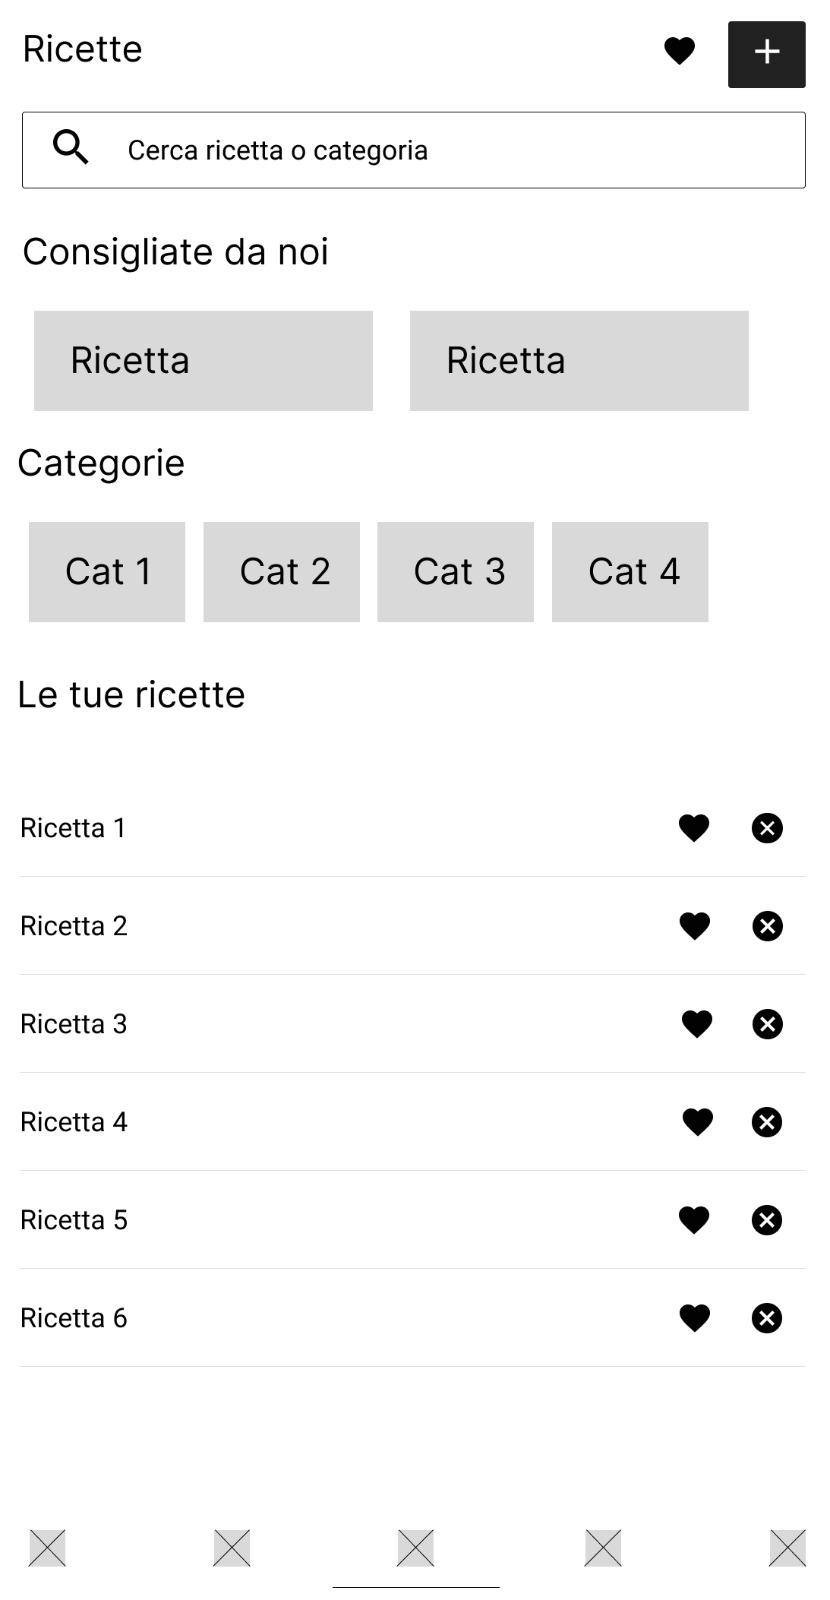
\includegraphics[width=\textwidth]{immage/Ricette.jpeg}
        \caption{Wireframe di Ricette}
    \end{minipage}
    \hfill
    \begin{minipage}{0.45\textwidth}
        \centering
        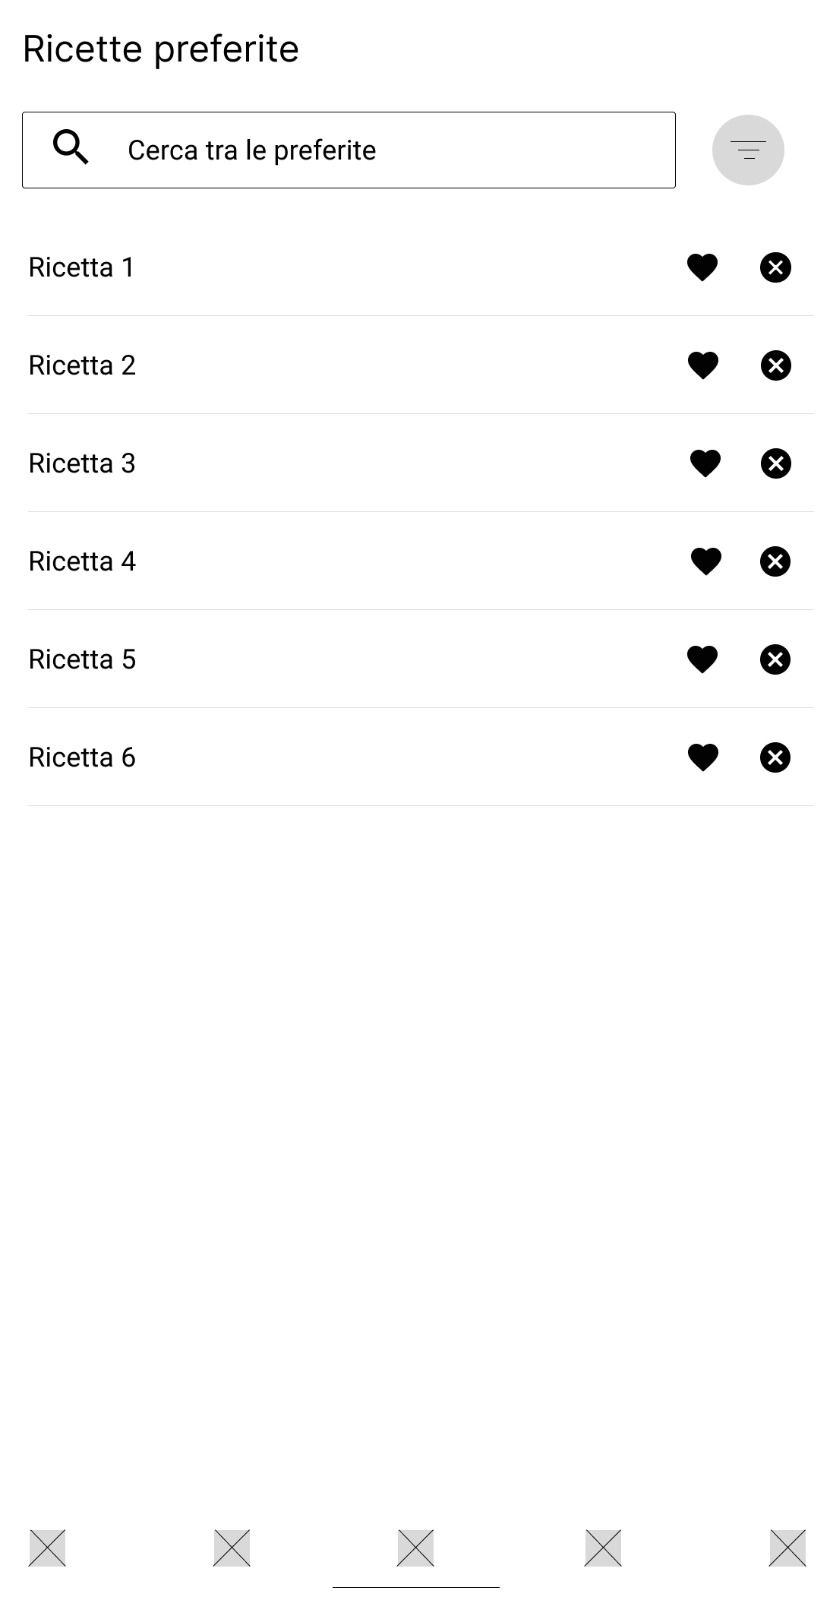
\includegraphics[width=\textwidth]{immage/Ricette-Preferite.jpeg}
        \caption{Wireframe di Ricette-Preferite}
    \end{minipage}
\end{figure}

\newpage

\begin{figure}[H]
    \vspace{3 cm}
    \centering
    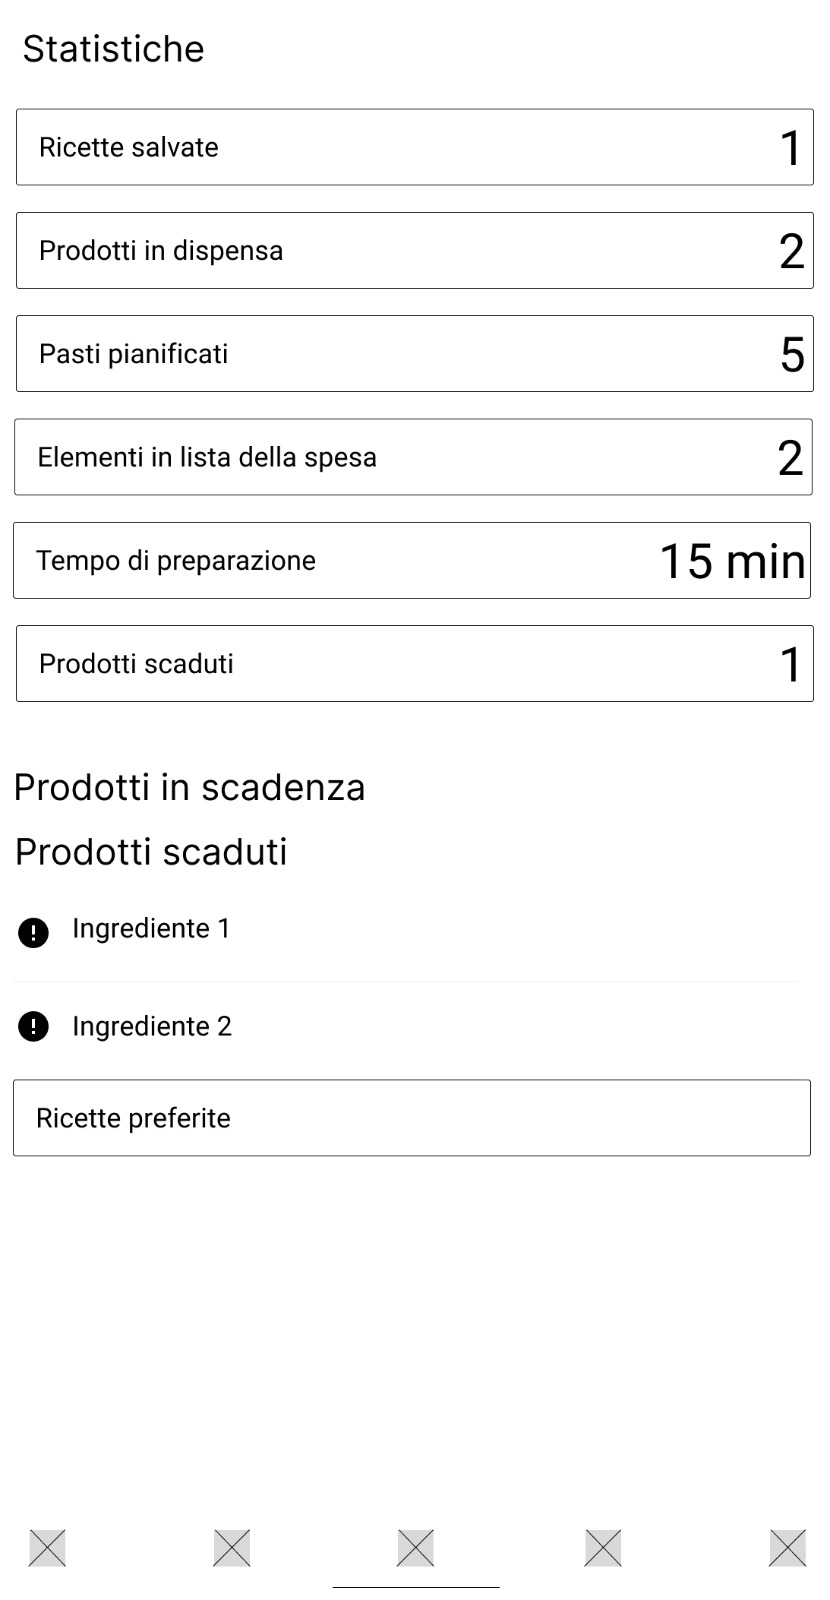
\includegraphics[width=0.5\textwidth]{immage/Statistiche.jpeg}
    \caption{Wireframe della pagina Statistiche}
\end{figure}



%--- seconda tabella ----
\newpage
\subsection{Organizzazione dei Dati}
\normalsize Dati dell’app sono organizzati in \textbf{5 entità principali}:
\begin{table}[H]
    \centering
    \renewcommand{\arraystretch}{1.5}
    \begin{tabularx}{\textwidth}{@{} >{\bfseries}l >{\centering}X >{\raggedright\arraybackslash}X @{}}
        \toprule
        \textbf{Entità} & \textbf{Persistenza} & \textbf{Campi principali} \\

        \midrule
        Recipe & SQLite & id, name, description, category, preparationTime, difficulty, portions, notes, imagePath, isRecommended, isFavorite \\
        \addlinespace
        RecipeIngredient & SQLite & id, recipeId (FK), name, quantity, unit\\
        \addlinespace
        PantryItem & SharedPreferences & id, name, category, quantity, unit, expiryDate, notes\\
        \addlinespace
        MealPlanItem & SharedPreferences & id, weekStart, day, mealType, recipeId\\
        \addlinespace
        ShoppingItem & SharedPreferences & id, name, quantity, unit, purchased\\
        
        \bottomrule 
    \end{tabularx}
    \caption{Tabella riassuntiva dell'organizzazione dei dati}
    \label{tab:requisiti_sistema}

\end{table}


% --- sezione 4 ---
\newpage
\section{Scelte tecnologiche}
\subsection{Framework utilizzato}
Flutter è stato scelto per la sua capacità di produrre app native ad alte prestazioni su iOS e Android a partire da un’unica codebase. \\
Il sistema di widget dichiarativi permette di costruire interfacce complesse in modo mantenibile. \\
Dart, il linguaggio sottostante, offre tipizzazione forte, null safety e asincronia tramite async/await, caratteristiche essenziali per un’app che gestisce I/O su database e file system.

\subsection{Librerie principali}
% -- tabella 3 

\begin{table}[H]
    \centering
    \renewcommand{\arraystretch}{1.5}
    \begin{tabularx}{\textwidth}{@{} >{\bfseries}l X @{}}
        \toprule
        \textbf{Libreria} & \textbf{Utilizzo} \\
        
        \midrule
        provider & Gestione dello stato globale tramite ChangeNotifier + Consumer pattern \\
        \addlinespace
        sqflite & Database SQLite locale per ricette e ingredienti con relazioni e foreign key \\
        \addlinespace
        shared\_preferences & Persistenza key-value per dispensa, meal plan e lista spesa in formato JSON \\
        \addlinespace
        path / path\_provider & Risoluzione del percorso del database SQLite sul filesystem del dispositivo \\
        \addlinespace
        image\_picker & Selezione immagine dalla galleria del dispositivo per le ricette \\
        \addlinespace
        intl & Formattazione delle date in formato dd/MM/yyyy nella schermata dispensa \\
        \addlinespace
        
        \bottomrule
    \end{tabularx}
    \caption{Schermate principali dell'applicazione}
    \label{tab:requisiti_sistema}

\end{table}

% --- Implementazione ---
\newpage
\section{Implementazione}


\subsection{Widget principali}
L’applicazione utilizza diversi widget e componenti personalizzati per implementare le funzionalità principali
\newline
\textbf{MainScreen} è un \textit{StatefulWidget} che ospita le cinque sezioni principali tramite \textit{IndexedStack}, che mantiene lo stato di ogni schermata attiva anche quando non visibile, evitando ricreazioni costose al cambio tab. \\
La navigazione tra tab avviene tramite \textit{BottomNavigationBar}.\\

\begin{itemize}
    \item IngredientRow
\end{itemize}
Classe di supporto utilizzata nel form delle ricette per gestire dinamicamente gli ingredienti.\\ 
Ogni riga contiene i controller per nome, quantità e unità di misura e può essere aggiunta o rimossa dall’utente durante la compilazione della ricetta.
\begin{itemize}
    \item Recipe Card
\end{itemize}
Componente utilizzato nella schermata \textbf{Ricette} per visualizzare sinteticamente le informazioni principali di una ricetta, tra cui nome, categoria, immagine e stato preferito.

\begin{itemize}[label=-]
    \item \textbf{ChoiceChip} utilizzato in \textit{RecipeFormScreen} per la selezione della difficoltà (Facile, Media, Difficile) e in \textit{FavoriteRecipesScreen} per i filtri avanzati nel bottom sheet. \\
    Permette una selezione visiva immediata tra opzioni mutualmente esclusive.
    \item \textbf{AlertDialog} riutilizzato in più contesti con comportamenti diversi: 
    \begin{itemize}[label=•]
        \item conferma eliminazione ricetta in RecipeDetailScreen.
        \item avviso ingredienti mancanti in MealPlanScreen.
        \item trasferimento prodotto in dispensa in ShoppingListScreen e modifica pasto in MealPlanScreen.
    \end{itemize}
    In tutti i casi con \textbf{StatefulBuilder} dove necessario per aggiornare lo stato interno.
    \item \textbf{ModalBottomSheet} con \textit{showDragHandle} in FavoriteRecipesScreen per il pannello filtri, che utilizza variabili temporanee per non applicare i filtri finché l'utente non preme "Applica", con possibilità di reset.
\end{itemize}

\newpage

\subsection{Organizzazione del codice}
Il progetto segue una struttura a layer chiaramente separati:
\begin{itemize}
    \item \textbf{\texttt{lib/models/}} → Classi dati pure (Recipe, RecipeIngredient, PantryItem, MealPlanItem, ShoppingItem) con metodi toJson/fromJson e toMap/fromMap per la serializzazione.
    \item \textbf{\texttt{lib/providers/}}  → AppState, unico provider di stato che espone i dati e i metodi di business logic a tutte le schermate.
    \item \textbf{\texttt{lib/database/}}  → DatabaseHelper, singleton che gestisce la connessione SQLite e tutte le operazioni sulle ricette.
    \item \textbf{\texttt{lib/screens/}}  → Tutte le schermate dell’app.
\end{itemize}

\subsection{Gestione della Navigazione}
La HomeScreen serve come punto di ingresso con accesso rapido a tutte le sezioni. 
Dalla HomeScreen, il tap su una voce apre MainScreen con il tab corrispondente pre-selezionato tramite il parametro initialIndex.
\vspace{0.5 cm}

La navigazione sfrutta due meccanismi:
\begin{itemize}
    \item \textbf{\texttt{Navigator.push()}} con MaterialPageRoute per le transizioni verso schermate secondarie (form, dettagli, preferite). \\ 
    Il ritorno avviene tramite \textbf{\texttt{Navigator.pop()}} o il tasto back del dispositivo.
    \item \textbf{\texttt{IndexedStack}} nella MainScreen per le cinque tab principali (Ricette, Dispensa, Meal Plan, Lista Spesa, Statistiche).\\
    Questo pattern mantiene lo stato di ogni schermata (scroll position, dati caricati) anche quando non è visibile, evitando ricreazioni costose.
\end{itemize}
\vspace{0.5 cm}

Il passaggio di dati tra schermate avviene in tre modi: 
\begin{enumerate}
    \item tramite costruttore (es. recipeId a RecipeDetailScreen).
    \item tramite Provider (accesso diretto ad AppState da qualsiasi schermata).
    \item tramite await su \textbf{\texttt{Navigator.push}} per aspettare il risultato di un form prima di aggiornare la UI.
\end{enumerate}

\newpage

\subsection{Gestione dello Stato}
AppState estende ChangeNotifier e viene iniettato nella widget tree tramite ChangeNotifierProvider al livello più alto dell’app.\\
Ogni schermata accede allo stato tramite Provider.of<AppState>(context) o Consumer<AppState>.\\

\vspace{0.5 cm}
Le operazioni che modificano lo stato seguono sempre il pattern:
\begin{itemize}[nosep]
    \item[] memoria → persistenza asincrona su disco → notifyListeners() per aggiornare la UI. Questo garantisce che la UI sia sempre sincronizzata con i dati persistiti.
\end{itemize}

\vspace{0.5 cm}
Per le ricette, che risiedono su SQLite, il pattern è leggermente diverso:
\begin{itemize}[nosep]
    \item[] l’operazione sul database viene completata prima di ricaricare la lista aggiornata tramite loadRecipesFromDatabase(), evitando stati inconsistenti.
\end{itemize}

\subsection{Gestione della Persistenza}
La scelta di usare \textbf{due sistemi} di persistenza distinti è motivata dalla natura dei dati:
\begin{itemize}
    \item \textbf{SQLite} per le ricette e i loro ingredienti: le ricette e i loro ingredienti sono salvati su SQLite con una relazione uno-a-molti(ON DELETE CASCADE).\\
    SQLite gestisce nativamente join, query filtrate e integrità referenziale con le foreign key e le operazioni CASCADE. La versione del database è predisposta tramite \_upgradeDB per supportare migrazioni future.
    \item \textbf{SharedPreferences} per gli altri dati: dispensa, meal plan e lista spesa sono liste piatte senza relazioni tra loro. \\
    La serializzazione JSON su SharedPreferences è più semplice da implementare e sufficientemente performante per le dimensioni tipiche di questi dataset.
\end{itemize}

Entrambe le soluzioni garantiscono la persistenza dei dati tra sessioni dell’app senza richiedere connettività o backend remoti.

\newpage
\subsection{Parti di codice significative o complesse}
{\color{ForestGreen}\raggedright{\textbf{Generazione Automatica della Lista della Spesa}}}\\
Il metodo \textbf{\texttt{generateShoppingListFromMealPlan()}} in \textbf{AppState} implementa la logica più complessa dell’app. \\
Per ogni pasto nel meal plan, recupera la ricetta associata e itera sugli ingredienti.\\
Prima di aggiungere un ingrediente alla lista, il sistema confronta gli ingredienti richiesti dalle ricette pianificate con quelli presenti in dispensa, considerando nome, unità di misura e quantità disponibile.\\
Se la quantità presente è insufficiente, viene aggiunta alla lista della spesa soltanto la quantità mancante\\
Mentre se l’ingrediente è già nella lista della spesa con la stessa unità, somma le quantità invece di duplicare la voce. \\
Questo approccio evita ridondanze e produce una lista spesa ottimizzata e pulita.
\newline

\vspace{0.5 cm}
\hrule
\vspace{0.5 cm}

{\color{ForestGreen}\raggedright{\textbf{Database SQLite con Relazione Uno-a-Molti}}}\\
La gestione del database in \textbf{\texttt{DatabaseHelper}} affronta il problema classico delle relazioni in SQLite. \\
L’operazione "getRecipes()" esegue prima una query sulla tabella recipes, poi per ogni ricetta una query secondaria su recipe\_ingredients filtrata per recipeId. \\
Questa strategia è accettabile per le dimensioni tipiche di un ricettario personale e mantiene il codice semplice e leggibile.
\newline

\vspace{0.5 cm}
\hrule
\vspace{0.5 cm}

{\color{ForestGreen}\raggedright{\textbf{Form Ingredienti Dinamico}}}\\
\textbf{\texttt{RecipeFormScreen}} implementa un sistema di righe ingredienti completamente dinamico tramite la classe di supporto \textbf{\texttt{IngredientRow}}, che incapsula i tre \textbf{\texttt{TextEditingController}} di ogni riga (nome, quantità, unità). \\
Il metodo dispose() di ogni \textbf{\texttt{IngredientRow}} viene richiamato correttamente quando la riga viene rimossa o quando il form viene chiuso, prevenendo memory leak.
\newline

\vspace{0.5 cm}
\hrule
\vspace{0.5 cm}

{\color{ForestGreen}\raggedright{\textbf{Suggerimento Ricette}}}\\
Il metodo suggestedRecipes() in AppState restituisce le ricette che hanno almeno un ingrediente presente in dispensa oppure che sono state marcate come raccomandate (isRecommended). \\
Le ricette raccomandate vengono mostrate con priorità e il numero massimo di suggerimenti visualizzati è limitato a cinque. \\
Il confronto avviene per nome normalizzato \textbf{\texttt{(toLowerCase().trim())}} per gestire variazioni di maiuscolo/minuscolo e spazi.
\newline

\newpage

{\color{ForestGreen}\raggedright{\textbf{Trasferimento Lista Spesa → Dispensa}}}\\
La funzione \textbf{\texttt{showAddToPantryDialog()}} in \textbf{\texttt{ShoppingListScreen}} implementa un \textbf{\texttt{dialog}} contestuale che appare quando l’utente preme il tasto elimina su un elemento della lista. \\
Il \textbf{\texttt{dialog}} propone di aggiungere il prodotto in dispensa con categoria, note e data di scadenza, oppure di eliminarlo semplicemente. \\
Questo aumenta la semplicità con cui è possibile tenere la dispensa aggiornata dopo la spesa.





\section{Conclusione}
Il progetto ha consentito di applicare i principali concetti affrontati durante il corso di \textbf{Mobile Programming}, tra cui gestione dello stato, navigazione, persistenza locale, progettazione dell'interfaccia utente e organizzazione del codice.\\
L'applicazione sviluppata risulta completa, estendibile e utilizzabile in un contesto reale per la pianificazione dei pasti e la gestione della dispensa domestica. 

\end{document}